Figure \ref{fig:error_distributions} shows the distribution of rotation and
translation errors across all experiments for all tested algorithms.

\begin{figure*}
\begin{framed}
  \vspace{-0.75cm}\hspace{-0.75cm}
    \subfloat{\definecolor{ccsm}{RGB}{228,26,28}
\definecolor{cndt}{RGB}{55,126,184}
\definecolor{cfgi}{RGB}{255,0,255}
\definecolor{cfvg}{RGB}{152,78,163}
\definecolor{cpso}{RGB}{255,127,0}
\definecolor{cfsm}{RGB}{77,175,74}
% GNUPLOT: LaTeX picture with Postscript
\begingroup
  \makeatletter
  \providecommand\color[2][]{%
    \GenericError{(gnuplot) \space\space\space\@spaces}{%
      Package color not loaded in conjunction with
      terminal option `colourtext'%
    }{See the gnuplot documentation for explanation.%
    }{Either use 'blacktext' in gnuplot or load the package
      color.sty in LaTeX.}%
    \renewcommand\color[2][]{}%
  }%
  \providecommand\includegraphics[2][]{%
    \GenericError{(gnuplot) \space\space\space\@spaces}{%
      Package graphicx or graphics not loaded%
    }{See the gnuplot documentation for explanation.%
    }{The gnuplot epslatex terminal needs graphicx.sty or graphics.sty.}%
    \renewcommand\includegraphics[2][]{}%
  }%
  \providecommand\rotatebox[2]{#2}%
  \@ifundefined{ifGPcolor}{%
    \newif\ifGPcolor
    \GPcolorfalse
  }{}%
  \@ifundefined{ifGPblacktext}{%
    \newif\ifGPblacktext
    \GPblacktexttrue
  }{}%
  % define a \g@addto@macro without @ in the name:
  \let\gplgaddtomacro\g@addto@macro
  % define empty templates for all commands taking text:
  \gdef\gplbacktext{}%
  \gdef\gplfronttext{}%
  \makeatother
  \ifGPblacktext
    % no textcolor at all
    \def\colorrgb#1{}%
    \def\colorgray#1{}%
  \else
    % gray or color?
    \ifGPcolor
      \def\colorrgb#1{\color[rgb]{#1}}%
      \def\colorgray#1{\color[gray]{#1}}%
      \expandafter\def\csname LTw\endcsname{\color{white}}%
      \expandafter\def\csname LTb\endcsname{\color{black}}%
      \expandafter\def\csname LTa\endcsname{\color{black}}%
      \expandafter\def\csname LT0\endcsname{\color[rgb]{1,0,0}}%
      \expandafter\def\csname LT1\endcsname{\color[rgb]{0,1,0}}%
      \expandafter\def\csname LT2\endcsname{\color[rgb]{0,0,1}}%
      \expandafter\def\csname LT3\endcsname{\color[rgb]{1,0,1}}%
      \expandafter\def\csname LT4\endcsname{\color[rgb]{0,1,1}}%
      \expandafter\def\csname LT5\endcsname{\color[rgb]{1,1,0}}%
      \expandafter\def\csname LT6\endcsname{\color[rgb]{0,0,0}}%
      \expandafter\def\csname LT7\endcsname{\color[rgb]{1,0.3,0}}%
      \expandafter\def\csname LT8\endcsname{\color[rgb]{0.5,0.5,0.5}}%
    \else
      % gray
      \def\colorrgb#1{\color{black}}%
      \def\colorgray#1{\color[gray]{#1}}%
      \expandafter\def\csname LTw\endcsname{\color{white}}%
      \expandafter\def\csname LTb\endcsname{\color{black}}%
      \expandafter\def\csname LTa\endcsname{\color{black}}%
      \expandafter\def\csname LT0\endcsname{\color{black}}%
      \expandafter\def\csname LT1\endcsname{\color{black}}%
      \expandafter\def\csname LT2\endcsname{\color{black}}%
      \expandafter\def\csname LT3\endcsname{\color{black}}%
      \expandafter\def\csname LT4\endcsname{\color{black}}%
      \expandafter\def\csname LT5\endcsname{\color{black}}%
      \expandafter\def\csname LT6\endcsname{\color{black}}%
      \expandafter\def\csname LT7\endcsname{\color{black}}%
      \expandafter\def\csname LT8\endcsname{\color{black}}%
    \fi
  \fi
    \setlength{\unitlength}{0.0500bp}%
    \ifx\gptboxheight\undefined%
      \newlength{\gptboxheight}%
      \newlength{\gptboxwidth}%
      \newsavebox{\gptboxtext}%
    \fi%
    \setlength{\fboxrule}{0.5pt}%
    \setlength{\fboxsep}{1pt}%
\begin{picture}(5000.00,8000.00)%
    \gplgaddtomacro\gplbacktext{%
      \colorrgb{0.15,0.15,0.15}%
      \put(518,6802){\makebox(0,0)[r]{\strut{}$10^{-2}$}}%
      \colorrgb{0.15,0.15,0.15}%
      \put(518,6951){\makebox(0,0)[r]{\strut{}$10^{-1}$}}%
      \colorrgb{0.15,0.15,0.15}%
      \put(518,7101){\makebox(0,0)[r]{\strut{}$10^0$}}%
      \colorrgb{0.15,0.15,0.15}%
      \put(518,7250){\makebox(0,0)[r]{\strut{}$10^1$}}%
      \colorrgb{0.15,0.15,0.15}%
      \put(518,7399){\makebox(0,0)[r]{\strut{}$10^2$}}%
    }%
    \gplgaddtomacro\gplfronttext{%
      \colorrgb{0.00,0.00,0.00}%
      \put(2587,7519){\makebox(0,0){\strut{}\scriptsize $(\overline{\delta}_{xy}, \overline{\delta}_\theta) = (0.05 \ \text{m}, 2 \ \text{deg})$}}%
      \put(2270,7800){\makebox(0,0){\strut{}{\color{ccsm}{\rule[0.6mm]{0.5cm}{0.5mm}}} \footnotesize CSM}}
      \put(3170,7800){\makebox(0,0){\strut{}{\color{cndt}{\rule[0.6mm]{0.5cm}{0.5mm}}} \footnotesize NDT}}
      \put(4240,7800){\makebox(0,0){\strut{}{\color{cfgi}{\rule[0.6mm]{0.5cm}{0.5mm}}} \footnotesize FastGICP}}
      \put(5400,7800){\makebox(0,0){\strut{}{\color{cfvg}{\rule[0.6mm]{0.5cm}{0.5mm}}} \footnotesize FastVGICP}}
      \put(6600,7800){\makebox(0,0){\strut{}{\color{cpso}{\rule[0.6mm]{0.5cm}{0.5mm}}} \footnotesize NDT-PSO}}
      \put(7600,7800){\makebox(0,0){\strut{}{\color{cfsm}{\rule[0.6mm]{0.5cm}{0.5mm}}} \footnotesize FSM}}
    }%
    \gplgaddtomacro\gplbacktext{%
      \colorrgb{0.15,0.15,0.15}%
      \put(518,5854){\makebox(0,0)[r]{\strut{}$10^{-2}$}}%
      \colorrgb{0.15,0.15,0.15}%
      \put(518,6003){\makebox(0,0)[r]{\strut{}$10^{-1}$}}%
      \colorrgb{0.15,0.15,0.15}%
      \put(518,6153){\makebox(0,0)[r]{\strut{}$10^0$}}%
      \colorrgb{0.15,0.15,0.15}%
      \put(518,6302){\makebox(0,0)[r]{\strut{}$10^1$}}%
      \colorrgb{0.15,0.15,0.15}%
      \put(518,6451){\makebox(0,0)[r]{\strut{}$10^2$}}%
    }%
    \gplgaddtomacro\gplfronttext{%
      \colorrgb{0.00,0.00,0.00}%
      \put(2587,6571){\makebox(0,0){\strut{}\scriptsize $(\overline{\delta}_{xy}, \overline{\delta}_\theta) = (0.10 \ \text{m}, 4 \ \text{deg})$}}%
    }%
    \gplgaddtomacro\gplbacktext{%
      \colorrgb{0.15,0.15,0.15}%
      \put(518,4907){\makebox(0,0)[r]{\strut{}$10^{-2}$}}%
      \colorrgb{0.15,0.15,0.15}%
      \put(518,5056){\makebox(0,0)[r]{\strut{}$10^{-1}$}}%
      \colorrgb{0.15,0.15,0.15}%
      \put(518,5206){\makebox(0,0)[r]{\strut{}$10^0$}}%
      \colorrgb{0.15,0.15,0.15}%
      \put(518,5355){\makebox(0,0)[r]{\strut{}$10^1$}}%
      \colorrgb{0.15,0.15,0.15}%
      \put(518,5504){\makebox(0,0)[r]{\strut{}$10^2$}}%
    }%
    \gplgaddtomacro\gplfronttext{%
      \colorrgb{0.15,0.15,0.15}%
      \put(-52,4705){\rotatebox{90}{\makebox(0,0){\strut{}Distribution of orientation errors [deg]}}}%
      \colorrgb{0.00,0.00,0.00}%
      \put(2587,5624){\makebox(0,0){\strut{}\scriptsize $(\overline{\delta}_{xy}, \overline{\delta}_\theta) = (0.15 \ \text{m}, 8.6 \ \text{deg})$}}%
    }%
    \gplgaddtomacro\gplbacktext{%
      \colorrgb{0.15,0.15,0.15}%
      \put(518,3959){\makebox(0,0)[r]{\strut{}$10^{-2}$}}%
      \colorrgb{0.15,0.15,0.15}%
      \put(518,4108){\makebox(0,0)[r]{\strut{}$10^{-1}$}}%
      \colorrgb{0.15,0.15,0.15}%
      \put(518,4258){\makebox(0,0)[r]{\strut{}$10^0$}}%
      \colorrgb{0.15,0.15,0.15}%
      \put(518,4407){\makebox(0,0)[r]{\strut{}$10^1$}}%
      \colorrgb{0.15,0.15,0.15}%
      \put(518,4556){\makebox(0,0)[r]{\strut{}$10^2$}}%
    }%
    \gplgaddtomacro\gplfronttext{%
      \colorrgb{0.00,0.00,0.00}%
      \put(2587,4676){\makebox(0,0){\strut{}\scriptsize $(\overline{\delta}_{xy}, \overline{\delta}_\theta) = (0.20 \ \text{m}, 17.2 \ \text{deg})$}}%
    }%
    \gplgaddtomacro\gplbacktext{%
      \colorrgb{0.15,0.15,0.15}%
      \put(518,3011){\makebox(0,0)[r]{\strut{}$10^{-2}$}}%
      \colorrgb{0.15,0.15,0.15}%
      \put(518,3161){\makebox(0,0)[r]{\strut{}$10^{-1}$}}%
      \colorrgb{0.15,0.15,0.15}%
      \put(518,3310){\makebox(0,0)[r]{\strut{}$10^0$}}%
      \colorrgb{0.15,0.15,0.15}%
      \put(518,3460){\makebox(0,0)[r]{\strut{}$10^1$}}%
      \colorrgb{0.15,0.15,0.15}%
      \put(518,3609){\makebox(0,0)[r]{\strut{}$10^2$}}%
    }%
    \gplgaddtomacro\gplfronttext{%
      \colorrgb{0.00,0.00,0.00}%
      \put(2587,3729){\makebox(0,0){\strut{}\scriptsize $(\overline{\delta}_{xy}, \overline{\delta}_\theta) = (0.20 \ \text{m}, 32 \ \text{deg})$}}%
    }%
    \gplgaddtomacro\gplbacktext{%
      \colorrgb{0.15,0.15,0.15}%
      \put(518,2064){\makebox(0,0)[r]{\strut{}$10^{-2}$}}%
      \colorrgb{0.15,0.15,0.15}%
      \put(518,2213){\makebox(0,0)[r]{\strut{}$10^{-1}$}}%
      \colorrgb{0.15,0.15,0.15}%
      \put(518,2363){\makebox(0,0)[r]{\strut{}$10^0$}}%
      \colorrgb{0.15,0.15,0.15}%
      \put(518,2512){\makebox(0,0)[r]{\strut{}$10^1$}}%
      \colorrgb{0.15,0.15,0.15}%
      \put(518,2661){\makebox(0,0)[r]{\strut{}$10^2$}}%
      \colorrgb{0.15,0.15,0.15}%
      \put(1037,1844){\makebox(0,0){\strut{}$0.01$}}%
      \colorrgb{0.15,0.15,0.15}%
      \put(1812,1844){\makebox(0,0){\strut{}$0.03$}}%
      \colorrgb{0.15,0.15,0.15}%
      \put(2587,1844){\makebox(0,0){\strut{}$0.05$}}%
      \colorrgb{0.15,0.15,0.15}%
      \put(3362,1844){\makebox(0,0){\strut{}$0.10$}}%
      \colorrgb{0.15,0.15,0.15}%
      \put(4137,1844){\makebox(0,0){\strut{}$0.20$}}%
    }%
    \gplgaddtomacro\gplfronttext{%
      \colorrgb{0.15,0.15,0.15}%
      \put(2587,1514){\makebox(0,0){\strut{}sd of sensor measurement noise $\sigma_R$ [m]}}%
      \colorrgb{0.00,0.00,0.00}%
      \put(2587,2781){\makebox(0,0){\strut{}\scriptsize $(\overline{\delta}_{xy}, \overline{\delta}_\theta) = (0.20 \ \text{m}, 45 \ \text{deg})$}}%
    }%
    \gplbacktext
    \put(0,0){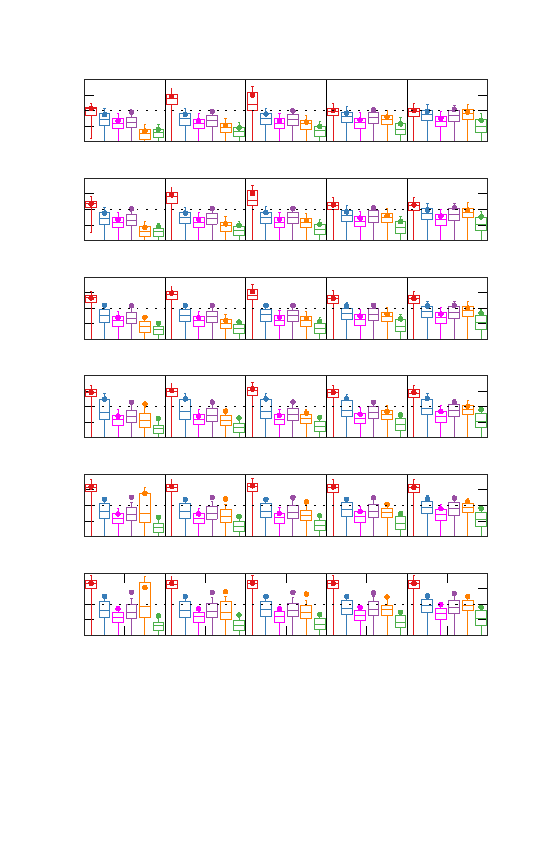
\includegraphics{./figures/experiments/orientation_errors}}%
    \gplfronttext
  \end{picture}%
\endgroup
}
    \qquad \hspace{-1.25cm}
    \subfloat{\definecolor{ccsm}{RGB}{228,26,28}
\definecolor{cndt}{RGB}{55,126,184}
\definecolor{cfgi}{RGB}{255,0,255}
\definecolor{cfvg}{RGB}{152,78,163}
\definecolor{cpso}{RGB}{255,127,0}
\definecolor{cfsm}{RGB}{77,175,74}

% GNUPLOT: LaTeX picture with Postscript
\begingroup
  \makeatletter
  \providecommand\color[2][]{%
    \GenericError{(gnuplot) \space\space\space\@spaces}{%
      Package color not loaded in conjunction with
      terminal option `colourtext'%
    }{See the gnuplot documentation for explanation.%
    }{Either use 'blacktext' in gnuplot or load the package
      color.sty in LaTeX.}%
    \renewcommand\color[2][]{}%
  }%
  \providecommand\includegraphics[2][]{%
    \GenericError{(gnuplot) \space\space\space\@spaces}{%
      Package graphicx or graphics not loaded%
    }{See the gnuplot documentation for explanation.%
    }{The gnuplot epslatex terminal needs graphicx.sty or graphics.sty.}%
    \renewcommand\includegraphics[2][]{}%
  }%
  \providecommand\rotatebox[2]{#2}%
  \@ifundefined{ifGPcolor}{%
    \newif\ifGPcolor
    \GPcolorfalse
  }{}%
  \@ifundefined{ifGPblacktext}{%
    \newif\ifGPblacktext
    \GPblacktexttrue
  }{}%
  % define a \g@addto@macro without @ in the name:
  \let\gplgaddtomacro\g@addto@macro
  % define empty templates for all commands taking text:
  \gdef\gplbacktext{}%
  \gdef\gplfronttext{}%
  \makeatother
  \ifGPblacktext
    % no textcolor at all
    \def\colorrgb#1{}%
    \def\colorgray#1{}%
  \else
    % gray or color?
    \ifGPcolor
      \def\colorrgb#1{\color[rgb]{#1}}%
      \def\colorgray#1{\color[gray]{#1}}%
      \expandafter\def\csname LTw\endcsname{\color{white}}%
      \expandafter\def\csname LTb\endcsname{\color{black}}%
      \expandafter\def\csname LTa\endcsname{\color{black}}%
      \expandafter\def\csname LT0\endcsname{\color[rgb]{1,0,0}}%
      \expandafter\def\csname LT1\endcsname{\color[rgb]{0,1,0}}%
      \expandafter\def\csname LT2\endcsname{\color[rgb]{0,0,1}}%
      \expandafter\def\csname LT3\endcsname{\color[rgb]{1,0,1}}%
      \expandafter\def\csname LT4\endcsname{\color[rgb]{0,1,1}}%
      \expandafter\def\csname LT5\endcsname{\color[rgb]{1,1,0}}%
      \expandafter\def\csname LT6\endcsname{\color[rgb]{0,0,0}}%
      \expandafter\def\csname LT7\endcsname{\color[rgb]{1,0.3,0}}%
      \expandafter\def\csname LT8\endcsname{\color[rgb]{0.5,0.5,0.5}}%
    \else
      % gray
      \def\colorrgb#1{\color{black}}%
      \def\colorgray#1{\color[gray]{#1}}%
      \expandafter\def\csname LTw\endcsname{\color{white}}%
      \expandafter\def\csname LTb\endcsname{\color{black}}%
      \expandafter\def\csname LTa\endcsname{\color{black}}%
      \expandafter\def\csname LT0\endcsname{\color{black}}%
      \expandafter\def\csname LT1\endcsname{\color{black}}%
      \expandafter\def\csname LT2\endcsname{\color{black}}%
      \expandafter\def\csname LT3\endcsname{\color{black}}%
      \expandafter\def\csname LT4\endcsname{\color{black}}%
      \expandafter\def\csname LT5\endcsname{\color{black}}%
      \expandafter\def\csname LT6\endcsname{\color{black}}%
      \expandafter\def\csname LT7\endcsname{\color{black}}%
      \expandafter\def\csname LT8\endcsname{\color{black}}%
    \fi
  \fi
    \setlength{\unitlength}{0.0500bp}%
    \ifx\gptboxheight\undefined%
      \newlength{\gptboxheight}%
      \newlength{\gptboxwidth}%
      \newsavebox{\gptboxtext}%
    \fi%
    \setlength{\fboxrule}{0.5pt}%
    \setlength{\fboxsep}{1pt}%
\begin{picture}(5000.00,8000.00)%
    \gplgaddtomacro\gplbacktext{%
      \colorrgb{0.15,0.15,0.15}%
      \put(518,6802){\makebox(0,0)[r]{\strut{}$0.0$}}%
      \colorrgb{0.15,0.15,0.15}%
      \colorrgb{0.15,0.15,0.15}%
      \put(518,7001){\makebox(0,0)[r]{\strut{}$0.10$}}%
      \colorrgb{0.15,0.15,0.15}%
      \colorrgb{0.15,0.15,0.15}%
      \put(518,7200){\makebox(0,0)[r]{\strut{}$0.20$}}%
      \colorrgb{0.15,0.15,0.15}%
      \colorrgb{0.15,0.15,0.15}%
      \put(518,7399){\makebox(0,0)[r]{\strut{}$0.30$}}%
    }%
    \gplgaddtomacro\gplfronttext{%
      \colorrgb{0.00,0.00,0.00}%
      \put(2587,7519){\makebox(0,0){\strut{}\scriptsize $(\overline{\delta}_{xy}, \overline{\delta}_\theta) = (0.05 \ \text{m}, 2 \ \text{deg})$}}%

      %\put(2270,8000){\makebox(0,0){\strut{}{\color{ccsm}{\rule[0.6mm]{0.5cm}{0.5mm}}} \footnotesize CSM}}
      %\put(3170,8000){\makebox(0,0){\strut{}{\color{cndt}{\rule[0.6mm]{0.5cm}{0.5mm}}} \footnotesize NDT}}
      %\put(4040,8000){\makebox(0,0){\strut{}{\color{cfgi}{\rule[0.6mm]{0.5cm}{0.5mm}}} \footnotesize FastGICP}}
      %\put(2100,7800){\makebox(0,0){\strut{}{\color{cfvg}{\rule[0.6mm]{0.5cm}{0.5mm}}} \footnotesize FastVGICP}}
      %\put(3200,7800){\makebox(0,0){\strut{}{\color{cpso}{\rule[0.6mm]{0.5cm}{0.5mm}}} \footnotesize NDT-PSO}}
      %\put(4170,7800){\makebox(0,0){\strut{}{\color{cfsm}{\rule[0.6mm]{0.5cm}{0.5mm}}} \footnotesize FSM}}
    }%
    \gplgaddtomacro\gplbacktext{%
      \colorrgb{0.15,0.15,0.15}%
      \put(518,5854){\makebox(0,0)[r]{\strut{}$0.0$}}%
      \colorrgb{0.15,0.15,0.15}%
      \colorrgb{0.15,0.15,0.15}%
      \put(518,6053){\makebox(0,0)[r]{\strut{}$0.10$}}%
      \colorrgb{0.15,0.15,0.15}%
      \colorrgb{0.15,0.15,0.15}%
      \put(518,6252){\makebox(0,0)[r]{\strut{}$0.20$}}%
      \colorrgb{0.15,0.15,0.15}%
      \colorrgb{0.15,0.15,0.15}%
      \put(518,6451){\makebox(0,0)[r]{\strut{}$0.30$}}%
    }%
    \gplgaddtomacro\gplfronttext{%
      \colorrgb{0.00,0.00,0.00}%
      \put(2587,6571){\makebox(0,0){\strut{}\scriptsize $(\overline{\delta}_{xy}, \overline{\delta}_\theta) = (0.10 \ \text{m}, 4 \ \text{deg})$}}%
    }%
    \gplgaddtomacro\gplbacktext{%
      \colorrgb{0.15,0.15,0.15}%
      \put(518,4907){\makebox(0,0)[r]{\strut{}$0.0$}}%
      \colorrgb{0.15,0.15,0.15}%
      \colorrgb{0.15,0.15,0.15}%
      \put(518,5078){\makebox(0,0)[r]{\strut{}$0.10$}}%
      \colorrgb{0.15,0.15,0.15}%
      \colorrgb{0.15,0.15,0.15}%
      \put(518,5248){\makebox(0,0)[r]{\strut{}$0.20$}}%
      \colorrgb{0.15,0.15,0.15}%
      \colorrgb{0.15,0.15,0.15}%
      \put(518,5419){\makebox(0,0)[r]{\strut{}$0.30$}}%
      \colorrgb{0.15,0.15,0.15}%
    }%
    \gplgaddtomacro\gplfronttext{%
      \colorrgb{0.15,0.15,0.15}%
      \put(-52,4705){\rotatebox{90}{\makebox(0,0){\strut{}Distribution of location errors [m]}}}%
      \colorrgb{0.00,0.00,0.00}%
      \put(2587,5624){\makebox(0,0){\strut{}\scriptsize $(\overline{\delta}_{xy}, \overline{\delta}_\theta) = (0.15 \ \text{m}, 8.6 \ \text{deg})$}}%
    }%
    \gplgaddtomacro\gplbacktext{%
      \colorrgb{0.15,0.15,0.15}%
      \put(518,3959){\makebox(0,0)[r]{\strut{}$0.0$}}%
      \colorrgb{0.15,0.15,0.15}%
      \colorrgb{0.15,0.15,0.15}%
      \put(518,4130){\makebox(0,0)[r]{\strut{}$0.10$}}%
      \colorrgb{0.15,0.15,0.15}%
      \colorrgb{0.15,0.15,0.15}%
      \put(518,4300){\makebox(0,0)[r]{\strut{}$0.20$}}%
      \colorrgb{0.15,0.15,0.15}%
      \colorrgb{0.15,0.15,0.15}%
      \put(518,4471){\makebox(0,0)[r]{\strut{}$0.30$}}%
      \colorrgb{0.15,0.15,0.15}%
    }%
    \gplgaddtomacro\gplfronttext{%
      \colorrgb{0.00,0.00,0.00}%
      \put(2587,4676){\makebox(0,0){\strut{}\scriptsize $(\overline{\delta}_{xy}, \overline{\delta}_\theta) = (0.20 \ \text{m}, 17.2 \ \text{deg})$}}%
    }%
    \gplgaddtomacro\gplbacktext{%
      \colorrgb{0.15,0.15,0.15}%
      \put(518,3011){\makebox(0,0)[r]{\strut{}$0.0$}}%
      \colorrgb{0.15,0.15,0.15}%
      \colorrgb{0.15,0.15,0.15}%
      \put(518,3182){\makebox(0,0)[r]{\strut{}$0.10$}}%
      \colorrgb{0.15,0.15,0.15}%
      \colorrgb{0.15,0.15,0.15}%
      \put(518,3353){\makebox(0,0)[r]{\strut{}$0.20$}}%
      \colorrgb{0.15,0.15,0.15}%
      \put(518,3524){\makebox(0,0)[r]{\strut{}$0.30$}}%
      \colorrgb{0.15,0.15,0.15}%
    }%
    \gplgaddtomacro\gplfronttext{%
      \colorrgb{0.00,0.00,0.00}%
      \put(2587,3729){\makebox(0,0){\strut{}\scriptsize $(\overline{\delta}_{xy}, \overline{\delta}_\theta) = (0.20 \ \text{m}, 32 \ \text{deg})$}}%
    }%
    \gplgaddtomacro\gplbacktext{%
      \colorrgb{0.15,0.15,0.15}%
      \put(518,2064){\makebox(0,0)[r]{\strut{}$0.0$}}%
      \colorrgb{0.15,0.15,0.15}%
      \colorrgb{0.15,0.15,0.15}%
      \put(518,2235){\makebox(0,0)[r]{\strut{}$0.10$}}%
      \colorrgb{0.15,0.15,0.15}%
      \colorrgb{0.15,0.15,0.15}%
      \put(518,2405){\makebox(0,0)[r]{\strut{}$0.20$}}%
      \colorrgb{0.15,0.15,0.15}%
      \colorrgb{0.15,0.15,0.15}%
      \put(518,2576){\makebox(0,0)[r]{\strut{}$0.30$}}%
      \colorrgb{0.15,0.15,0.15}%
      \colorrgb{0.15,0.15,0.15}%
      \put(1037,1844){\makebox(0,0){\strut{}$0.01$}}%
      \colorrgb{0.15,0.15,0.15}%
      \put(1812,1844){\makebox(0,0){\strut{}$0.03$}}%
      \colorrgb{0.15,0.15,0.15}%
      \put(2587,1844){\makebox(0,0){\strut{}$0.05$}}%
      \colorrgb{0.15,0.15,0.15}%
      \put(3362,1844){\makebox(0,0){\strut{}$0.10$}}%
      \colorrgb{0.15,0.15,0.15}%
      \put(4137,1844){\makebox(0,0){\strut{}$0.20$}}%
    }%
    \gplgaddtomacro\gplfronttext{%
      \colorrgb{0.15,0.15,0.15}%
      \put(2587,1514){\makebox(0,0){\strut{}sd of sensor measurement noise $\sigma_R$ [m]}}%
      \colorrgb{0.00,0.00,0.00}%
      \put(2587,2781){\makebox(0,0){\strut{}\scriptsize $(\overline{\delta}_{xy}, \overline{\delta}_\theta) = (0.20 \ \text{m}, 45 \ \text{deg})$}}%
    }%
    \gplbacktext
    \put(0,0){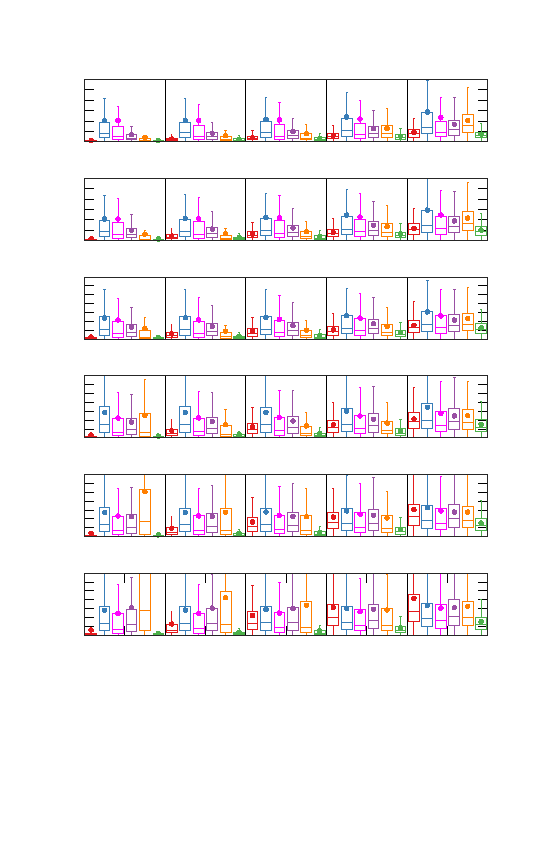
\includegraphics{./figures/experiments/position_errors}}%
    \gplfronttext
  \end{picture}%
\endgroup
}
    \vspace{-2.5cm}
    \caption{\small Distribution of orientation and position errors across a
             range of maximal positional and orientational displacements, for
             progressively larger sensor measurement noise levels. Each boxplot
             represents $10$ iterations over $\approx 45$$\cdot$$10^3$ random
             scan pairs for each configuration. FSM's errors are largely
             independent of the initial displacement of scans for a given level
             of sensor noise}%
    \label{fig:error_distributions}%
\end{framed}
\end{figure*}

\begin{figure}
\vspace{-0.75cm}\hspace{0.1cm}
    \definecolor{rr}{RGB}{119,172,48}
\definecolor{gg}{RGB}{162,20,47}
% GNUPLOT: LaTeX picture with Postscript
\begingroup
  \makeatletter
  \providecommand\color[2][]{%
    \GenericError{(gnuplot) \space\space\space\@spaces}{%
      Package color not loaded in conjunction with
      terminal option `colourtext'%
    }{See the gnuplot documentation for explanation.%
    }{Either use 'blacktext' in gnuplot or load the package
      color.sty in LaTeX.}%
    \renewcommand\color[2][]{}%
  }%
  \providecommand\includegraphics[2][]{%
    \GenericError{(gnuplot) \space\space\space\@spaces}{%
      Package graphicx or graphics not loaded%
    }{See the gnuplot documentation for explanation.%
    }{The gnuplot epslatex terminal needs graphicx.sty or graphics.sty.}%
    \renewcommand\includegraphics[2][]{}%
  }%
  \providecommand\rotatebox[2]{#2}%
  \@ifundefined{ifGPcolor}{%
    \newif\ifGPcolor
    \GPcolorfalse
  }{}%
  \@ifundefined{ifGPblacktext}{%
    \newif\ifGPblacktext
    \GPblacktexttrue
  }{}%
  % define a \g@addto@macro without @ in the name:
  \let\gplgaddtomacro\g@addto@macro
  % define empty templates for all commands taking text:
  \gdef\gplbacktext{}%
  \gdef\gplfronttext{}%
  \makeatother
  \ifGPblacktext
    % no textcolor at all
    \def\colorrgb#1{}%
    \def\colorgray#1{}%
  \else
    % gray or color?
    \ifGPcolor
      \def\colorrgb#1{\color[rgb]{#1}}%
      \def\colorgray#1{\color[gray]{#1}}%
      \expandafter\def\csname LTw\endcsname{\color{white}}%
      \expandafter\def\csname LTb\endcsname{\color{black}}%
      \expandafter\def\csname LTa\endcsname{\color{black}}%
      \expandafter\def\csname LT0\endcsname{\color[rgb]{1,0,0}}%
      \expandafter\def\csname LT1\endcsname{\color[rgb]{0,1,0}}%
      \expandafter\def\csname LT2\endcsname{\color[rgb]{0,0,1}}%
      \expandafter\def\csname LT3\endcsname{\color[rgb]{1,0,1}}%
      \expandafter\def\csname LT4\endcsname{\color[rgb]{0,1,1}}%
      \expandafter\def\csname LT5\endcsname{\color[rgb]{1,1,0}}%
      \expandafter\def\csname LT6\endcsname{\color[rgb]{0,0,0}}%
      \expandafter\def\csname LT7\endcsname{\color[rgb]{1,0.3,0}}%
      \expandafter\def\csname LT8\endcsname{\color[rgb]{0.5,0.5,0.5}}%
    \else
      % gray
      \def\colorrgb#1{\color{black}}%
      \def\colorgray#1{\color[gray]{#1}}%
      \expandafter\def\csname LTw\endcsname{\color{white}}%
      \expandafter\def\csname LTb\endcsname{\color{black}}%
      \expandafter\def\csname LTa\endcsname{\color{black}}%
      \expandafter\def\csname LT0\endcsname{\color{black}}%
      \expandafter\def\csname LT1\endcsname{\color{black}}%
      \expandafter\def\csname LT2\endcsname{\color{black}}%
      \expandafter\def\csname LT3\endcsname{\color{black}}%
      \expandafter\def\csname LT4\endcsname{\color{black}}%
      \expandafter\def\csname LT5\endcsname{\color{black}}%
      \expandafter\def\csname LT6\endcsname{\color{black}}%
      \expandafter\def\csname LT7\endcsname{\color{black}}%
      \expandafter\def\csname LT8\endcsname{\color{black}}%
    \fi
  \fi
    \setlength{\unitlength}{0.0500bp}%
    \ifx\gptboxheight\undefined%
      \newlength{\gptboxheight}%
      \newlength{\gptboxwidth}%
      \newsavebox{\gptboxtext}%
    \fi%
    \setlength{\fboxrule}{0.5pt}%
    \setlength{\fboxsep}{1pt}%
\begin{picture}(5000.00,6000.00)%
    \gplgaddtomacro\gplbacktext{%
    }%
    \gplgaddtomacro\gplfronttext{%
    }%
    \gplgaddtomacro\gplbacktext{%
    }%
    \gplgaddtomacro\gplfronttext{%
    }%
    \gplgaddtomacro\gplbacktext{%
    }%
    \gplgaddtomacro\gplfronttext{%
      \colorrgb{0.00,0.00,0.00}%
      \put(2587,4571){\makebox(0,0){\strut{}\small Colour signification of proportion of rays'}}%
      \put(2587,4391){\makebox(0,0){\strut{}\small ranges within maximum sensor range}}%

      \put(1970,3700){\makebox(0,0){\strut{}{\color{rr}{\rule[0.6mm]{0.5cm}{0.5mm}}} \footnotesize $\overline{\delta}_{xy} = 0.05$ m}}
      \put(3470,3700){\makebox(0,0){\strut{}{\color{gg}{\rule[0.6mm]{0.5cm}{0.5mm}}} \footnotesize $\overline{\delta}_{xy} = 0.20$ m}}
    }%
    \gplgaddtomacro\gplbacktext{%
    }%
    \gplgaddtomacro\gplfronttext{%
      \colorrgb{0.15,0.15,0.15}%
      \put(650,3980){\makebox(0,0){\strut{}\scriptsize $0\%$}}%
      \colorrgb{0.15,0.15,0.15}%
      \put(1425,3980){\makebox(0,0){\strut{}\scriptsize $20\%$}}%
      \colorrgb{0.15,0.15,0.15}%
      \put(2200,3980){\makebox(0,0){\strut{}\scriptsize $40\%$}}%
      \colorrgb{0.15,0.15,0.15}%
      \put(2974,3980){\makebox(0,0){\strut{}\scriptsize $60\%$}}%
      \colorrgb{0.15,0.15,0.15}%
      \put(3749,3980){\makebox(0,0){\strut{}\scriptsize $80\%$}}%
      \colorrgb{0.15,0.15,0.15}%
      \put(4524,3980){\makebox(0,0){\strut{}\scriptsize $100\%$}}%
    }%
    \gplgaddtomacro\gplbacktext{%
      \colorrgb{0.00,0.00,0.00}%
      \put(608,2700){\makebox(0,0)[r]{\strut{}$0.0$}}%
      \colorrgb{0.00,0.00,0.00}%
      \put(608,2962){\makebox(0,0)[r]{\strut{}$23.0$}}%
      \colorrgb{0.00,0.00,0.00}%
      \put(608,3224){\makebox(0,0)[r]{\strut{}$46.0$}}%
      \colorrgb{0.00,0.00,0.00}%
      \put(608,3486){\makebox(0,0)[r]{\strut{}$69.0$}}%
      \colorrgb{0.15,0.15,0.15}%
      \put(740,2480){\makebox(0,0){\strut{}}}%
      \colorrgb{0.15,0.15,0.15}%
      \put(1027,2480){\makebox(0,0){\strut{}}}%
      \colorrgb{0.15,0.15,0.15}%
      \put(1315,2480){\makebox(0,0){\strut{}}}%
      \colorrgb{0.15,0.15,0.15}%
      \put(1602,2480){\makebox(0,0){\strut{}}}%
      \colorrgb{0.15,0.15,0.15}%
      \put(1890,2480){\makebox(0,0){\strut{}}}%
      \colorrgb{0.15,0.15,0.15}%
      \put(2177,2480){\makebox(0,0){\strut{}}}%
    }%
    \gplgaddtomacro\gplfronttext{%
      \colorrgb{0.15,0.15,0.15}%
      \put(-58,3093){\rotatebox{90}{\makebox(0,0){\strut{}$e_{orient}$ [deg]}}}%
    }%
    \gplgaddtomacro\gplbacktext{%
      \colorrgb{0.00,0.00,0.00}%
      \put(2955,2700){\makebox(0,0)[r]{\strut{$0.0$}}}
      \colorrgb{0.00,0.00,0.00}%
      \put(2955,2925){\makebox(0,0)[r]{\strut{$23.0$}}}%
      \colorrgb{0.00,0.00,0.00}%
      \put(2955,3149){\makebox(0,0)[r]{\strut{$46.0$}}}%
      \colorrgb{0.00,0.00,0.00}%
      \put(2955,3374){\makebox(0,0)[r]{\strut{$69.0$}}}%
      \colorrgb{0.15,0.15,0.15}%
      \put(3087,2480){\makebox(0,0){\strut{}}}%
      \colorrgb{0.15,0.15,0.15}%
      \put(3374,2480){\makebox(0,0){\strut{}}}%
      \colorrgb{0.15,0.15,0.15}%
      \put(3662,2480){\makebox(0,0){\strut{}}}%
      \colorrgb{0.15,0.15,0.15}%
      \put(3949,2480){\makebox(0,0){\strut{}}}%
      \colorrgb{0.15,0.15,0.15}%
      \put(4237,2480){\makebox(0,0){\strut{}}}%
      \colorrgb{0.15,0.15,0.15}%
      \put(4524,2480){\makebox(0,0){\strut{}}}%
    }%
    \gplgaddtomacro\gplfronttext{%
    }%
    \gplgaddtomacro\gplbacktext{%
      \colorrgb{0.15,0.15,0.15}%
      \put(608,1560){\makebox(0,0)[r]{\strut{}\small $0.0$}}%
      \colorrgb{0.15,0.15,0.15}%
      \put(608,1757){\makebox(0,0)[r]{\strut{}\small $0.05$}}%
      \colorrgb{0.15,0.15,0.15}%
      \put(608,1953){\makebox(0,0)[r]{\strut{}\small $0.10$}}%
      \colorrgb{0.15,0.15,0.15}%
      \put(608,2150){\makebox(0,0)[r]{\strut{}\small $0.15$}}%
      \colorrgb{0.15,0.15,0.15}%
      \put(608,2346){\makebox(0,0)[r]{\strut{}\small $0.20$}}%
      \colorrgb{0.15,0.15,0.15}%
      \put(1027,1340){\makebox(0,0){\strut{}\small $20\%$}}%
      \colorrgb{0.15,0.15,0.15}%
      \put(1602,1340){\makebox(0,0){\strut{}\small $60\%$}}%
      \colorrgb{0.15,0.15,0.15}%
      \put(2177,1340){\makebox(0,0){\strut{}\small $100\%$}}%
    }%
    \gplgaddtomacro\gplfronttext{%
      \colorrgb{0.15,0.15,0.15}%
      \put(-58,1953){\rotatebox{90}{\makebox(0,0){\strut{}$e_{pos}$ [m]}}}%
    }%
    \gplgaddtomacro\gplbacktext{%
      \colorrgb{0.15,0.15,0.15}%
      \put(2955,1560){\makebox(0,0)[r]{\strut{}\small $0.0$}}%
      \colorrgb{0.15,0.15,0.15}%
      \put(2955,1757){\makebox(0,0)[r]{\strut{}\small $0.05$}}%
      \colorrgb{0.15,0.15,0.15}%
      \put(2955,1953){\makebox(0,0)[r]{\strut{}\small $0.10$}}%
      \colorrgb{0.15,0.15,0.15}%
      \put(2955,2150){\makebox(0,0)[r]{\strut{}\small $0.15$}}%
      \colorrgb{0.15,0.15,0.15}%
      \put(2955,2346){\makebox(0,0)[r]{\strut{}\small $0.20$}}%
      \colorrgb{0.15,0.15,0.15}%
      \put(3374,1340){\makebox(0,0){\strut{}\small $20\%$}}%
      \colorrgb{0.15,0.15,0.15}%
      \put(3949,1340){\makebox(0,0){\strut{}\small $60\%$}}%
      \colorrgb{0.15,0.15,0.15}%
      \put(4524,1340){\makebox(0,0){\strut{}\small $100\%$}}%
    }%
    \gplgaddtomacro\gplfronttext{%
    }%
    \gplbacktext
    \put(0,0){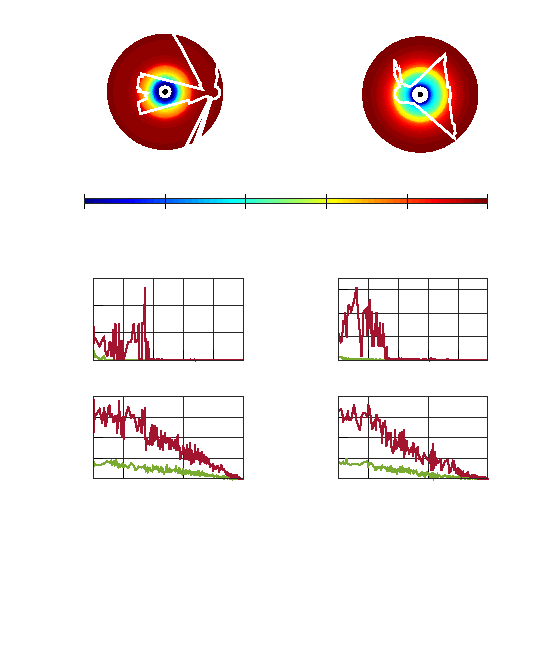
\includegraphics{./figures/experiments/max_range_test}}%
    \gplfronttext
  \end{picture}%
\endgroup

    \vspace{-2.5cm}
    \caption{FSM's performance with respect to receding maximum range}%
    \label{}%
\end{figure}

FSM's position and orientation errors are equal to or lower than the most
accurate method for each displacement and sensor noise configuration. As
displacements and sensor noise levels increase, its errors increase at a lower
rate than any tested method. The magnitude of FSM's errors is largely
independent of the displacement of the two input scans for a given level of
sensor noise (fig.  \ref{fig:laser_odometry}). The juxtaposition of the six
methods' errors at high levels of sensor noise highlight the robustness
afforded to FSM by the Discrete Fourier transform and its properties.

In terms of execution time, CSM ranged between $4.8$-$17.5$ ms, NDT
$8.1$-$19.9$ ms, FastGICP $3$-$9$ ms, FastVGICP $3.8$-$6.8$ ms,
NDT-PSO $190$-$200$ ms, and FSM between $13.2$ and $16.7$ ms.  The
measurement frequency of modern LIDAR sensors ranges from $12$-$20$ Hz;
therefore FSM runs in real time in modern processors.
